

\section{Analysis}
We now present our analysis of 
EU collected data. We concentrate our investigation 
along several directions. First, we investigate how frequently EU
requests are served from non-adequate destinations in each
source country.
We further analyze the prevalence of known third-party trackers
that are located in non-adequate destinations by source country.
While both of these scenarios constitute potential GDPR violations,
the latter is a stronger case since known trackers are more 
likely to be capturing personal information and 
by definition are sending such data to 
third parties.

Second, we analyze the most prevalent trackers, and the types of
websites that load them, in each source country.
Third, we investigate whether there are regional differences
across the EU in compliance with data localization.
Finally, we study the cookies loaded by sites that contact
non-adequate servers.


\subsection{Servers in Non-Adequate Countries}
\label{sec:analysis1}

We now turn to the question of prevalence of servers, generally,
and tracking servers, specifically, in non-adequate countries
by source EU country. 
Tab.~\ref{tab:countriesheat} shows a
summary of three key metrics in this regard. First, the
percentage of traceroutes sent from each EU country that reached
a server in a non-adequate country. Second, the percentage
of unique server IPs that are hosted in a non-adequate country,
and third, the same metric for unique tracking servers.

At a high level, we find that data localization is complied with
in the vast majority of cases, as evidenced by the low
percentages in all columns of Tab.~\ref{tab:countriesheat};
we present the last two columns as a geographic heatmap in  
in Fig.~\ref{fig:euheat}.
(In \S~\ref{sec:regionalvariation}, we investigate the 
apparent geographic trends in Fig.~\ref{fig:euheat}.)
However, since
we collected data from the most popular sites in each country,
the exceptions still represent potentially very large traffic volumes
from EU countries to non-adequate countries. For instance,
4.6\% of unique IPs that serve users in Poland are located
in a non-adequate country, and the same figure is 4.2\% for Greece.
Moreover, in a majority of the 20 EU countries we studied,
more than 1\% of third-party trackers are hosted 
in non-adequate destinations. (We further investigate 
these trackers in \S~\ref{sec:trackers}.)



\begin{table}
  \caption{Percentage of traceroutes, servers and trackers reaching non-adequate destination countries, by source EU country, sorted decreasingly on row average (not shown).}
  \label{tab:countriesheat}

\begin{tabular}{cccc}
    \toprule
    \textbf{Source Country} & \textbf{Traceroutes}  & \textbf{IPs} & \textbf{Unique} \\
     & \textbf{Unique} &  & \textbf{Tracker IPs} \\
    \toprule
    RO & \cellcolor{green!100}6.6 & \cellcolor{green!42.42}2.8 & \cellcolor{green!21.21}1.4 \\
    \midrule
    FI & \cellcolor{green!65.15}4.3 & \cellcolor{green!65.15}4.3 & \cellcolor{green!16.67}1.1 \\
    \midrule
    IT & \cellcolor{green!10.61}0.7 & \cellcolor{green!57.58}3.8 & \cellcolor{green!60.61}4.0 \\
    \midrule
    GR & \cellcolor{green!21.21}1.4 & \cellcolor{green!63.64}4.2 & \cellcolor{green!43.94}2.9 \\
    \midrule
    SK & \cellcolor{green!12.12}0.8 & \cellcolor{green!56.06}3.7 & \cellcolor{green!56.06}3.7 \\
    \midrule
    PL & \cellcolor{green!12.12}0.8 & \cellcolor{green!69.70}4.6 & \cellcolor{green!36.36}2.4 \\
    \midrule
    CZ & \cellcolor{green!4.55}0.3 & \cellcolor{green!53.03}3.5 & \cellcolor{green!12.12}0.8 \\
    \midrule
    ES & \cellcolor{green!6.06}0.4 & \cellcolor{green!34.85}2.3 & \cellcolor{green!24.24}1.6 \\
    \midrule
    HR & \cellcolor{green!13.64}0.9 & \cellcolor{green!25.76}1.7 & \cellcolor{green!24.24}1.6 \\
    \midrule
    HU & \cellcolor{green!6.06}0.4 & \cellcolor{green!27.27}1.8 & \cellcolor{green!30.30}2.0 \\
    \midrule
    AT & \cellcolor{green!9.09}0.6 & \cellcolor{green!25.76}1.7 & \cellcolor{green!18.18}1.2 \\
    \midrule
    DE & \cellcolor{green!9.09}0.6 & \cellcolor{green!31.82}2.1 & \cellcolor{green!7.58}0.5 \\
    \midrule
    PT & \cellcolor{green!6.06}0.4 & \cellcolor{green!18.18}1.2 & \cellcolor{green!19.70}1.3 \\
    \midrule
    NL & \cellcolor{green!3.03}0.2 & \cellcolor{green!19.70}1.3 & \cellcolor{green!21.21}1.4 \\
    \midrule
    IE & \cellcolor{green!13.64}0.9 & \cellcolor{green!21.21}1.4 & \cellcolor{green!7.58}0.5 \\
    \midrule
    BG & \cellcolor{green!3.03}0.2 & \cellcolor{green!16.67}1.1 & \cellcolor{green!21.21}1.4 \\
    \midrule
    FR & \cellcolor{green!6.06}0.4 & \cellcolor{green!19.70}1.3 & \cellcolor{green!6.06}0.4 \\
    \midrule
    SE & \cellcolor{green!4.55}0.3 & \cellcolor{green!19.70}1.3 & \cellcolor{green!6.06}0.4 \\
    \midrule
    DK & \cellcolor{green!1.52}0.1 & \cellcolor{green!3.03}0.2 & \cellcolor{green!0.00}0.0 \\
    \midrule
    BE & \cellcolor{green!1.52}0.1 & \cellcolor{green!1.52}0.1 & \cellcolor{green!0.00}0.0 \\
    \bottomrule
\end{tabular}
\end{table}


\begin{center}
\begin{figure}
    \centering
    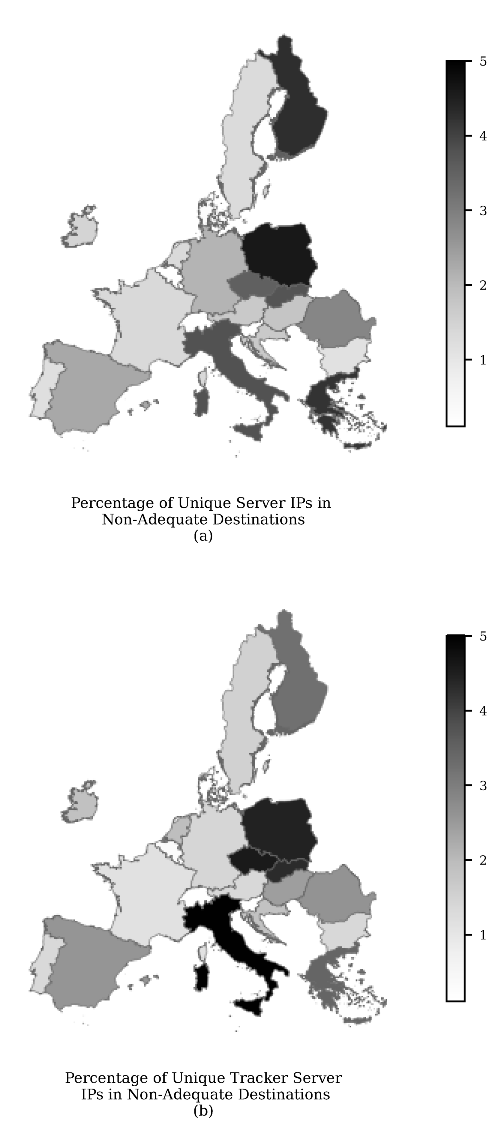
\includegraphics[width=0.8\linewidth]{figures/greece-uniquetrackeripandserver.pdf}
    \caption{Percentage of unique tracker IPs in non-adequate countries.}
\label{fig:euheat}
\vspace{-6mm}
\end{figure}
\end{center}


\subsection{Destination Countries}
The non-adequate destination countries in our sample
span several continents. 
In Tab.~\ref{tab:traceroutesheat} we show
those most commonly occuring among these countries.
The US, Turkey and Russia account for approximately 90\% of
traceroutes crossing from the EU into a non-adequate destination.
While the US is a relatively common destination for most EU
source countries, Russia and Turkey are much more prevalent in 
two nearby source countries: Finland and Romania, respectively.


\begin{table*}
  \caption{Number of traceroutes reaching top 10 non-adequate Countries (together they account for 97.7\% of these traceroutes).}
  \label{tab:traceroutesheat}

\begin{tabular}{ccccccccccccccccccccc}
    \toprule
     \textbf{Source} $\xrightarrow{}$ & \textbf{RO} & \textbf{FI} & \textbf{GR} & \textbf{HR} & \textbf{IE} & \textbf{PL} & \textbf{SK} & \textbf{IT} & \textbf{AT} & \textbf{DE} & \textbf{PT} & \textbf{FR} & \textbf{ES} & \textbf{HU} & \textbf{CZ} & \textbf{SE} & \textbf{NL} & \textbf{BG} & \textbf{BE} & \textbf{DK} \\
    
    \textbf{Destination} $\downarrow$ & & & & & & & & & & & & & & & & & & & \\
   
    \midrule
    \textbf{US} & \cellcolor{green!19}3 & \cellcolor{green!19}3 & \cellcolor{green!33}16 & \cellcolor{green!51}29 & \cellcolor{green!60}34 & \cellcolor{green!100}85 & \cellcolor{green!54}46 & \cellcolor{green!55}47 & \cellcolor{green!50}43 & \cellcolor{green!48}41 & \cellcolor{green!24}5 & \cellcolor{green!36}12 & \cellcolor{green!68}58 & \cellcolor{green!38}13 & \cellcolor{green!44}17 & \cellcolor{green!33}16 & \cellcolor{green!33}16 & \cellcolor{green!27}7 &  &  \\ 
    \midrule
    \textbf{TR} & \cellcolor{green!100}308 & \cellcolor{green!15}2 &  & \cellcolor{green!15}2 & \cellcolor{green!31}11 &  &  &  &  &  &  &  &  &  &  & \cellcolor{green!31}11 & \cellcolor{green!15}2 & \cellcolor{green!15}1 &  & \cellcolor{green!15}1 \\ 
    \midrule
    \textbf{RU} &  & \cellcolor{green!100}147 & \cellcolor{green!15}2 &  &  &  &  &  & \cellcolor{green!15}1 &  &  &  & \cellcolor{green!15}1 &  &  & \cellcolor{green!27}7 &  & \cellcolor{green!15}2 &  & \cellcolor{green!15}2 \\ 
    \midrule
    \textbf{MX} &  &  &  &  &  & \cellcolor{green!41}35 &  & \cellcolor{green!15}2 &  &  &  & \cellcolor{green!15}1 & \cellcolor{green!15}1 &  & \cellcolor{green!15}1 &  &  &  &  &  \\ 
    \midrule
    \textbf{IN} & \cellcolor{green!15}1 & \cellcolor{green!15}1 & \cellcolor{green!19}4 & \cellcolor{green!15}1 & \cellcolor{green!19}4 & \cellcolor{green!19}4 & \cellcolor{green!15}2 & \cellcolor{green!24}5 & \cellcolor{green!19}4 & \cellcolor{green!15}1 & \cellcolor{green!15}2 &  & \cellcolor{green!18}3 &  & \cellcolor{green!15}1 &  & \cellcolor{green!15}1 & \cellcolor{green!15}1 &  &  \\ 
    \midrule
    \textbf{SG} &  &  & \cellcolor{green!27}6 &  &  & \cellcolor{green!15}1 &  &  & \cellcolor{green!15}2 & \cellcolor{green!15}1 &  & \cellcolor{green!15}1 & \cellcolor{green!15}1 &  & \cellcolor{green!15}2 &  & \cellcolor{green!27}7 &  &  &  \\ 
    \midrule
    \textbf{HK} & \cellcolor{green!15}1 &  & \cellcolor{green!27}7 & \cellcolor{green!15}1 & \cellcolor{green!15}1 &  &  & \cellcolor{green!15}1 &  & \cellcolor{green!24}5 & \cellcolor{green!15}1 &  & \cellcolor{green!15}1 & \cellcolor{green!15}1 & \cellcolor{green!15}1 &  &  &  &  &  \\ 
    \midrule
    \textbf{BR} & \cellcolor{green!19}2 &  &  &  &  &  & \cellcolor{green!15}1 & \cellcolor{green!24}5 &  &  &  & \cellcolor{green!15}1 & \cellcolor{green!15}1 &  & \cellcolor{green!19}2 &  & \cellcolor{green!15}1 & \cellcolor{green!19}2 & \cellcolor{green!19}2 &  \\ 
    \midrule
    \textbf{AE} &  &  &  &  &  &  &  & \cellcolor{green!18}3 & \cellcolor{green!15}1 &  &  & \cellcolor{green!15}1 & \cellcolor{green!15}1 &  & \cellcolor{green!24}4 &  &  & \cellcolor{green!15}1 &  &  \\ 
    \midrule
    \textbf{AU} &  &  &  &  &  & \cellcolor{green!15}1 &  & \cellcolor{green!15}1 &  & \cellcolor{green!19}2 &  &  & \cellcolor{green!15}1 &  & \cellcolor{green!15}1 &  &  &  &  &  \\ 


    \bottomrule

\end{tabular}
\end{table*}



\subsection{Trackers}
\label{sec:trackers}
We now turn our attention to known third-party trackers. As
stated earlier, these domains are of particular concern from
a privacy standpoint because of their collection of
sensitive information from users, especially in cases
where it is transferred to non-adequate countries. 
We investigate three aspects of the trackers in non-adequate countries 
observed in our data:
the source-destination pairs of countries, the most commonly occurring trackers in 
each source EU country, and the most common types of websites that host the trackers.

\subsubsection{Source-Destination Country Pairs}
In Fig.~\ref{fig:flowsrcdst} we show the pairs of
source EU countries and non-adequate destination country in our
data; each flow is weighted by the 
number of traceroutes seen between each pair of countries. 
As observed before for traceroutes towards all
destinations (not just trackers), the US is also the most common destination
among trackers in non-adequate countries. The US is the 
most common destination from all but five EU countries in our
sample: Netherlands, Ireland, Czech Republic, Romania and Finland.

Four destination countries are also notable in Fig.~\ref{fig:flowsrcdst}.
India is observed as a destination from 13 EU countries; in over
80\% of cases (among 49 traceroutes), a Google (third-party) tracker is responsible
for this. Russia, Turkey and
Hong Kong are frequent destinations from three EU countries: Finland, Romania
and Greece, respectively. Thus, the trend observed earlier for all traceroutes
from the former two EU sources holds also for known trackers. 
A majority (26/43) of the traceroutes between Romania and Turkey are
caused by a single popular website: \textit{fandom.com},
a site focused on arts and entertainment ~\cite{SimilarWeb}.
In the case of Finland and Russia, exactly half (30/60) of
the traceroutes are caused by popular website \textit{vk.com},
a social media network~\cite{SimilarWeb} that is popular among Russian speakers.
(Russian speakers are a minority group in Finland, which borders Russia).
Finally, 17 of 19 traceroutes
from Greece to Hong Kong are caused by a single third-party tracker: Facebook, 
whoose trackers are loaded by 10 popular websites. \textit{makeleio.gr}, a news and
media publisher~\cite{SimilarWeb}, is the most commonly occurring popular website, responsible for 4/17 of
these traceroutes. 

\begin{figure}
    \centering
    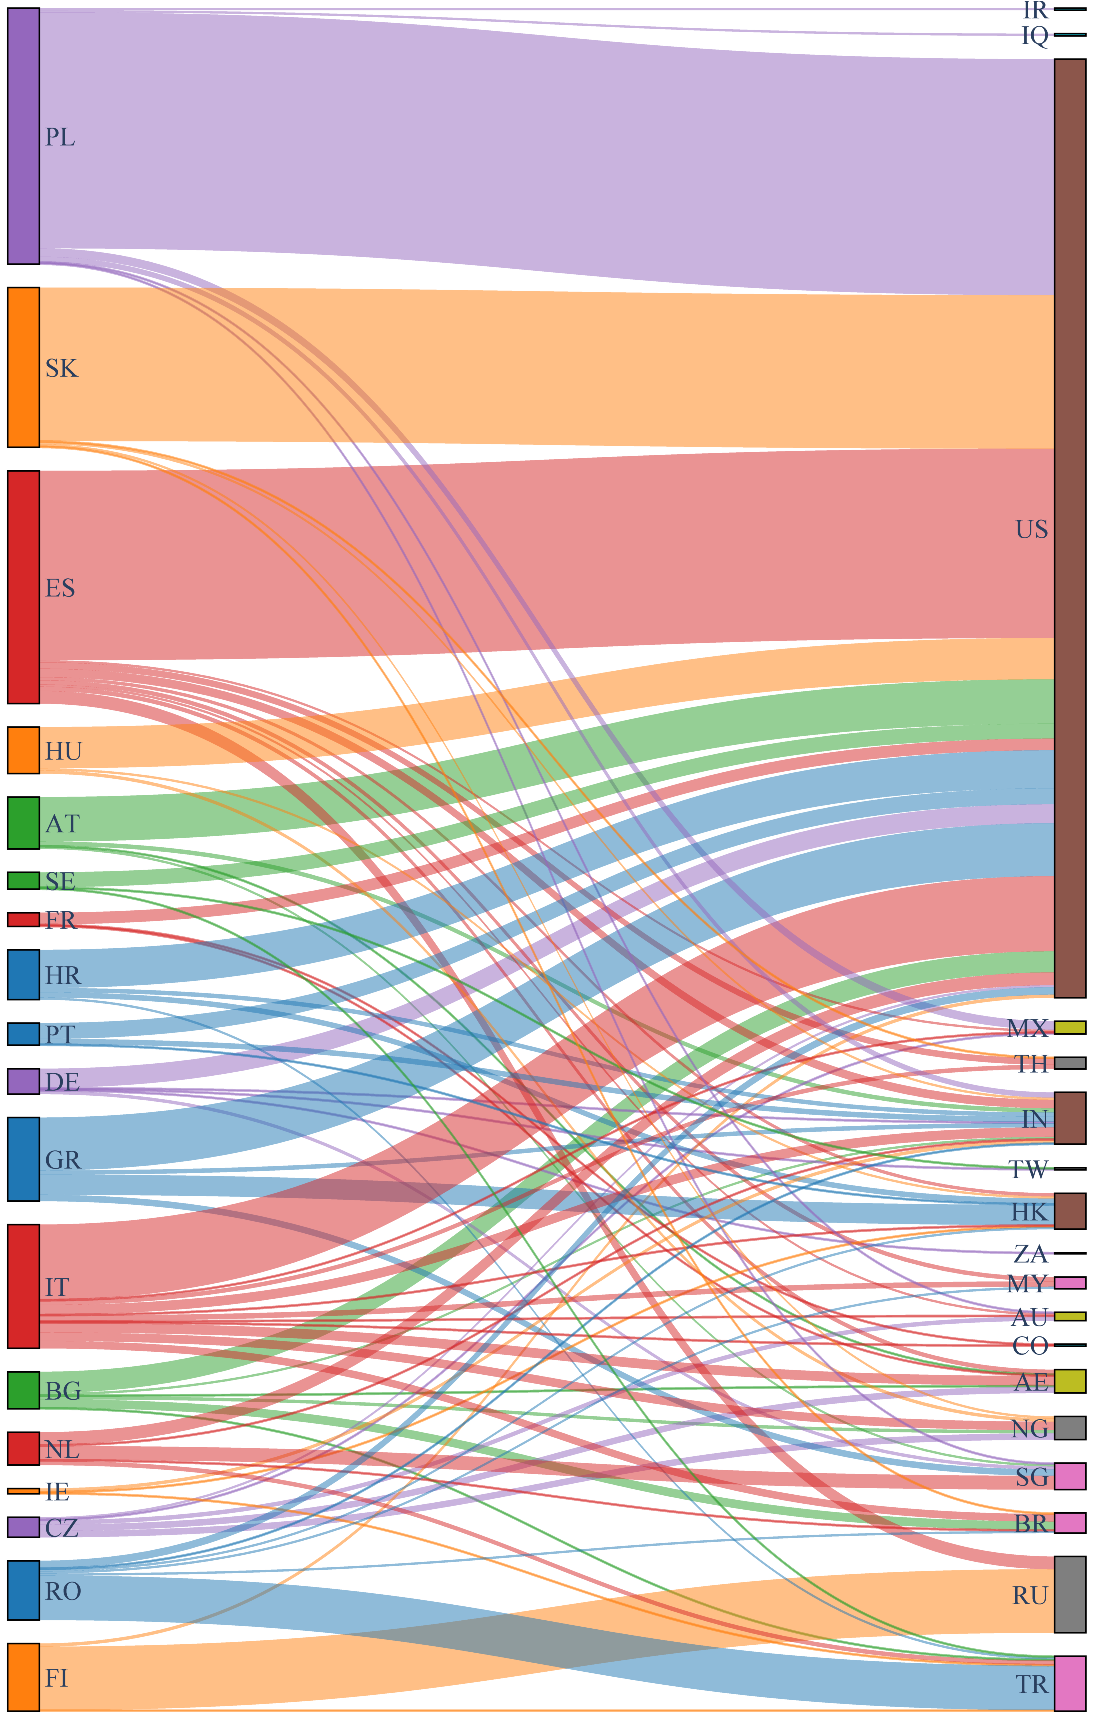
\includegraphics[width=\linewidth]{figures/src-dst-no-first-party.pdf}
    \caption{Flowchart showing, among 
known third-party trackers located in non-adequate countries, 
the prevalence of traceroutes connecting each source-destination pair of countries.}
\label{fig:flowsrcdst}
\end{figure}


\subsection{Common Paths}

We now investigate common paths that take a request from an EU country
to a non-adequate destination. We define a path as a combination of 
source country, initial website, tracker, and destination country. 
Among these paths, we show those that occur at least 5 times in our traceroute
set in Fig.~\ref{fig:flowcmmntrk}. Two of these paths, which originate in 
Romania and Finland through \textit{fandom.com} and \textit{vk.com}, respectively, were mentioned earlier.
(\textit{userapi.com} might be ``affiliated'' with \textit{vk.com}, but we could not
confirm the former's ownership by the latter, thus we classify this site as a third-party.)

At a high level, we observe a variety of paths that are not particularly concentrated 
among any one website or tracker. Notably, only four of these trackers seem to be operated by major
US companies: \textit{dailymotion.com}, \textit{gvt1.com} and \textit{gstatic.com} (Google), 
and \textit{clarity.ms} (Microsoft). As before, there are a wide variety of paths that reach the US 
through combinations of popular websites and trackers.

\begin{figure}
    \centering
    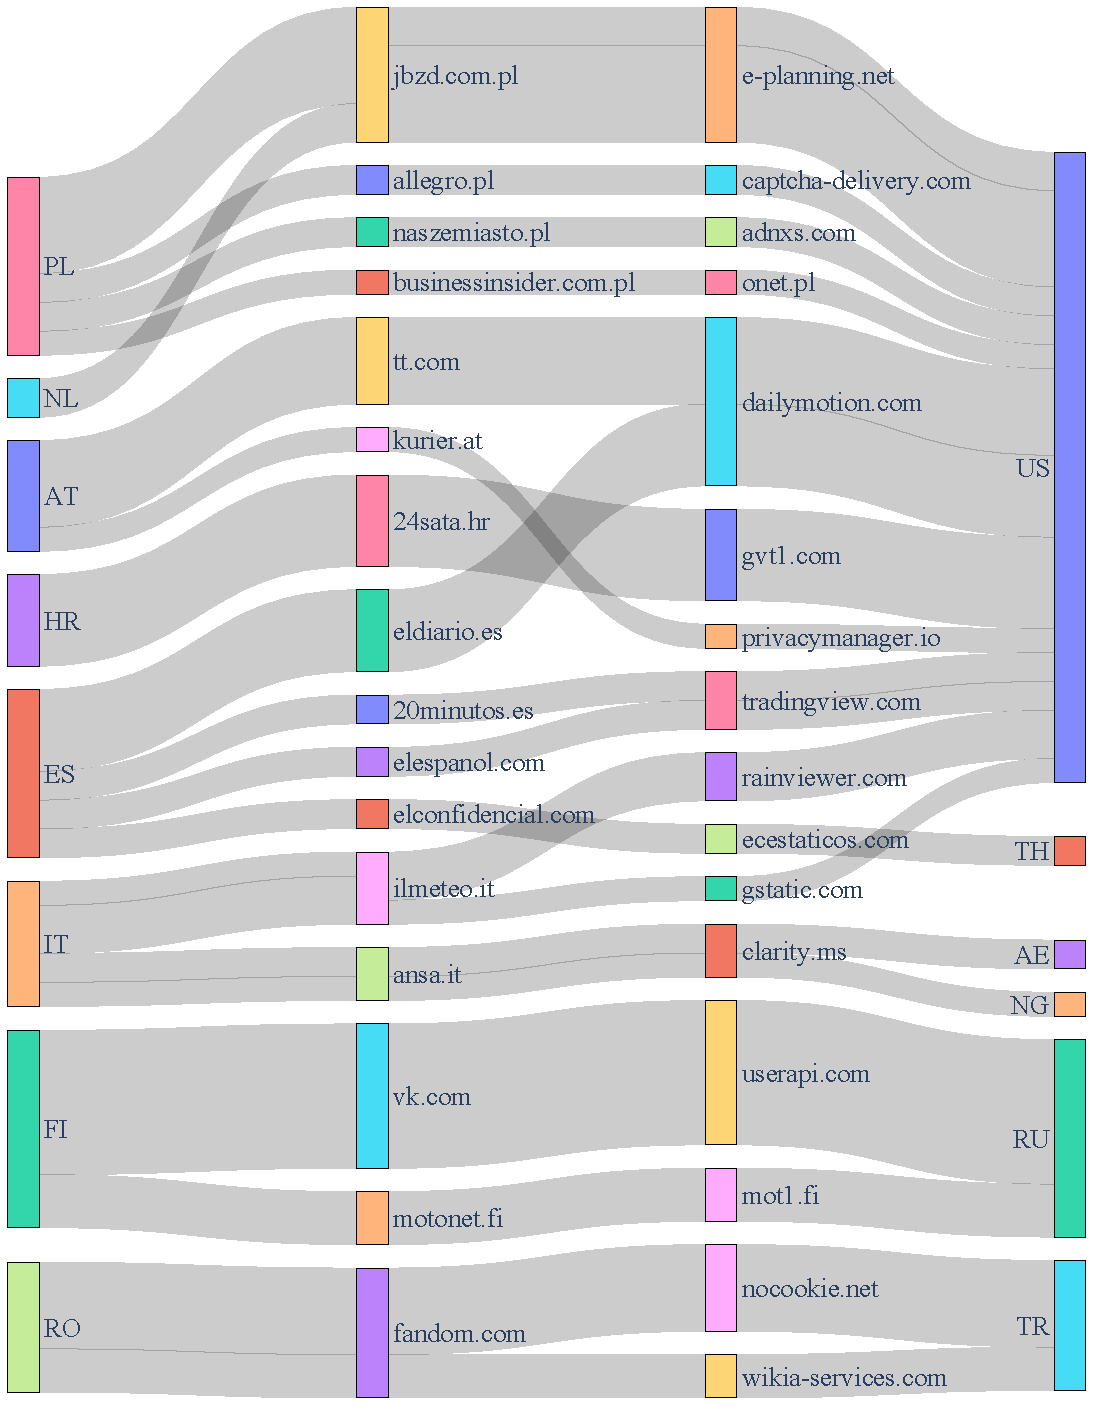
\includegraphics[width=\linewidth]{figures/full-flow-no-first-party-alteast-5-pairs.pdf}\\
    \caption{Combinations of
source country, initial website, third-party tracker, and destination country that are observed
five times or more in our data.}
\label{fig:flowcmmntrk}
\end{figure}


\subsection{Initial Website Categories}
\label{sec:categories}

We now turn to the question of which types of websites
are responsible for loading these third-party trackers in
non-adequate countries. Anectodally, news sites seem prevalent among these;
for instance, in Fig.~\ref{fig:flowcmmntrk}, all the initial websites in Spain
are news websites. 
We now systematically investigate whether that is broadly the case.
In Fig.~\ref{fig:categories} we
present the \textit{SimilarWeb} categories~\cite{SimilarWeb} associated with the 239 websites
that load at least one of these trackers. A slim majority of these sites, 120, 
belong to the News \& Media Publishers category (including the four aforementioned sites in Spain). 
This category makes intuitive sense
as a frequent fetcher of trackers due to the news industry's increasing reliance
on digital advertising revenue and thus on web tracking. Nevertheless, the high
prevalence of this category in the set of sites loading trackers in non-adequate countries is still notable.
For instance, three other categories include at least 20 websites: Arts \& Entertainment, Computers Electronics and Technology,
and Ecommerce \& Shopping. However, none of them come close to the prevalence of News \& Media Publishers.

\begin{figure}[t]
    \centering
    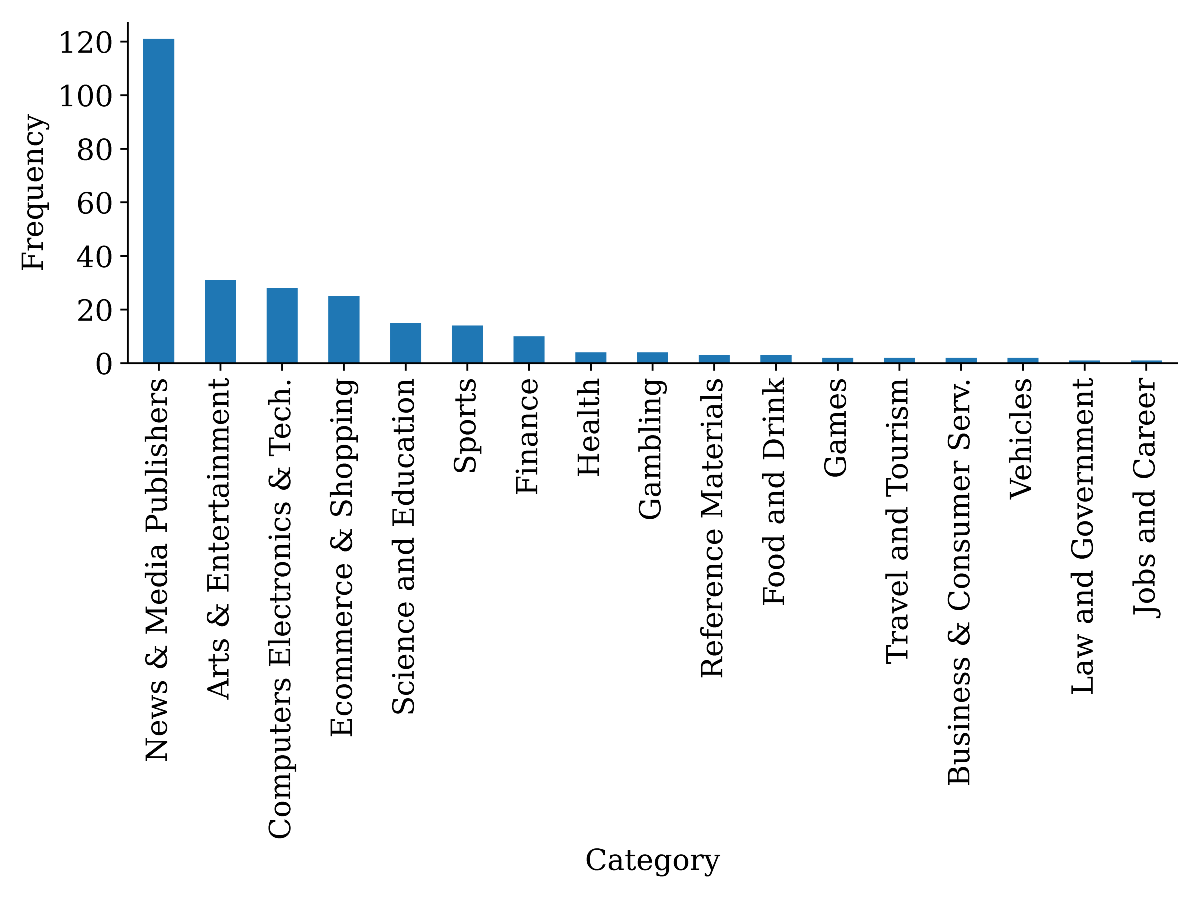
\includegraphics[width=\linewidth]{figures/bar-plot-category.pdf}\\
    \caption{Categories for websites that load observed trackers in non-adequate destinations.}
\label{fig:categories}
\end{figure}


\subsection{Regional Variation}
\label{sec:regionalvariation}
In previous subsections, especially in 
Fig.~\ref{fig:euheat}, we anecdotally observed that the rates of 
servers located in non-adequate countries seemed higher in Southern and
Eastern Europe. To evaluate whether this is true, systematically,
we use the United Nations defition~\cite{uneu} for four regions of Europe: 
Northern, Southern, Eastern and Western.
We evaluate both the rate of server IPs, overall, and tracker IPs, specifically.

The findings are shown in Fig.~\ref{fig:regional}. The rates
of presence in non-adequate countries is higher in Southern and Eastern 
Europe, compared with Northern and Western Europe, for both server IPs and tracker IPs. 
We use an ANOVA test to determine whether these regional differences are statistically significant.
For server IPs, they are not ($p=0.19$). For tracker IPs, however, the difference is significant ($p=0.01$).
This latter category presents bigger privacy risks.
This disparity can lead to higher risks of privacy harms for users in Eastern and Southern Europe.

\begin{figure}
    \centering
    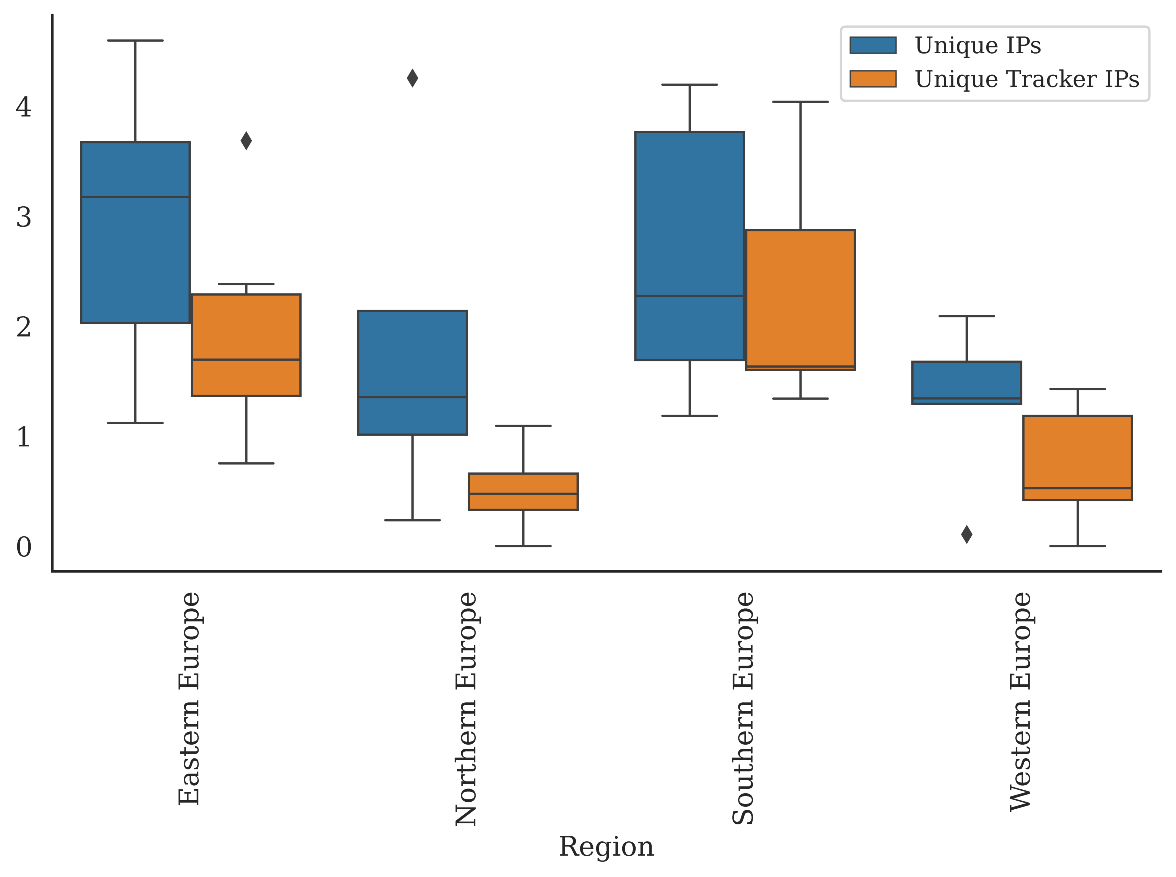
\includegraphics[width=\linewidth]{figures/boxplot.pdf}
    \caption{Boxplots showing the percentage of non-adequate server IPs and tracker IPs for the countries 
present in each EU region.}
\label{fig:regional}
\end{figure}

\subsection{Cookies}
In this subsection, we present an analysis of the cookies that were
loaded by initial sites that contacted at least one server in a non-adequate country.
We find substantial evidence that servers in non-adequate countries 
are engaging in user tracking activities.

Of the 1,233 non-adequate instances observed in \S~\ref{subsec:finalsample}
(recall that an instance is an initial site loaded from an ASCP),
we find that 824 retrieve and store non-empty cookies. 
Of these, 236 websites load cookies with unique identifiers, for a total of 9,885 cookies. 
Unique identifiers pose a potential privacy harm, as they can be used to track
users beyond the website they are currently browsing.
These cookies contain 1,153 unique identifiers. 
The unique identifiers~\cite{munir2023cookiegraph} in a cookie's name or value 
can provide valuable context about the organization that issued or uses the cookie. 
We also used Cookiedatabase~\cite{cookiedatabase} for identifying organizations based on the unique identifier.
We found 494 cookies that contain an identifer $\texttt{\_ga}$, 
which indicates they were set by Google Analytics. 
Similarly, 457 cookies have $\texttt{\_gid}$ and 254 have $\texttt{\_\_gfp\_64b}$, which indicates 
they are used by Google services for analytics and ad personalization (DoubleClick), respectively.

Other popular cookie identifier were, $\texttt{\_fbp}$ (230 cookies), 
set by Facebook for marketing. Additionally, we observed various identifiers 
that are related to consent management such as \path{\_pbjs\_userid\_consent\_data} and $\texttt{OptanonConsent}$.  
Consent management ensures compliance with privacy regulations by enabling users to control their data collection preferences.
Figure ~\ref{fig:cookie_website}(a) illustrates the distribution of the most frequently observed cookies.


Our analysis also identified the most commonly occurring cookies across websites. 
The most frequent cookie was $\texttt{\_ga}$ (Google Analytics), found on 146 websites, 
followed by $\texttt{\_gid}$ (Google Analytics) on 135 websites, $\texttt{\_\_gfp\_64b}$ (Doubleclick) 
on 84 and $\texttt{\_fbp}$ (Facebook) on 63 websites. 
Figures~\ref{fig:cookie_website}(b) illustrates and highlights the prevalence of tracking and analytics cookies across websites.





\begin{center}
\begin{figure}
    \centering
    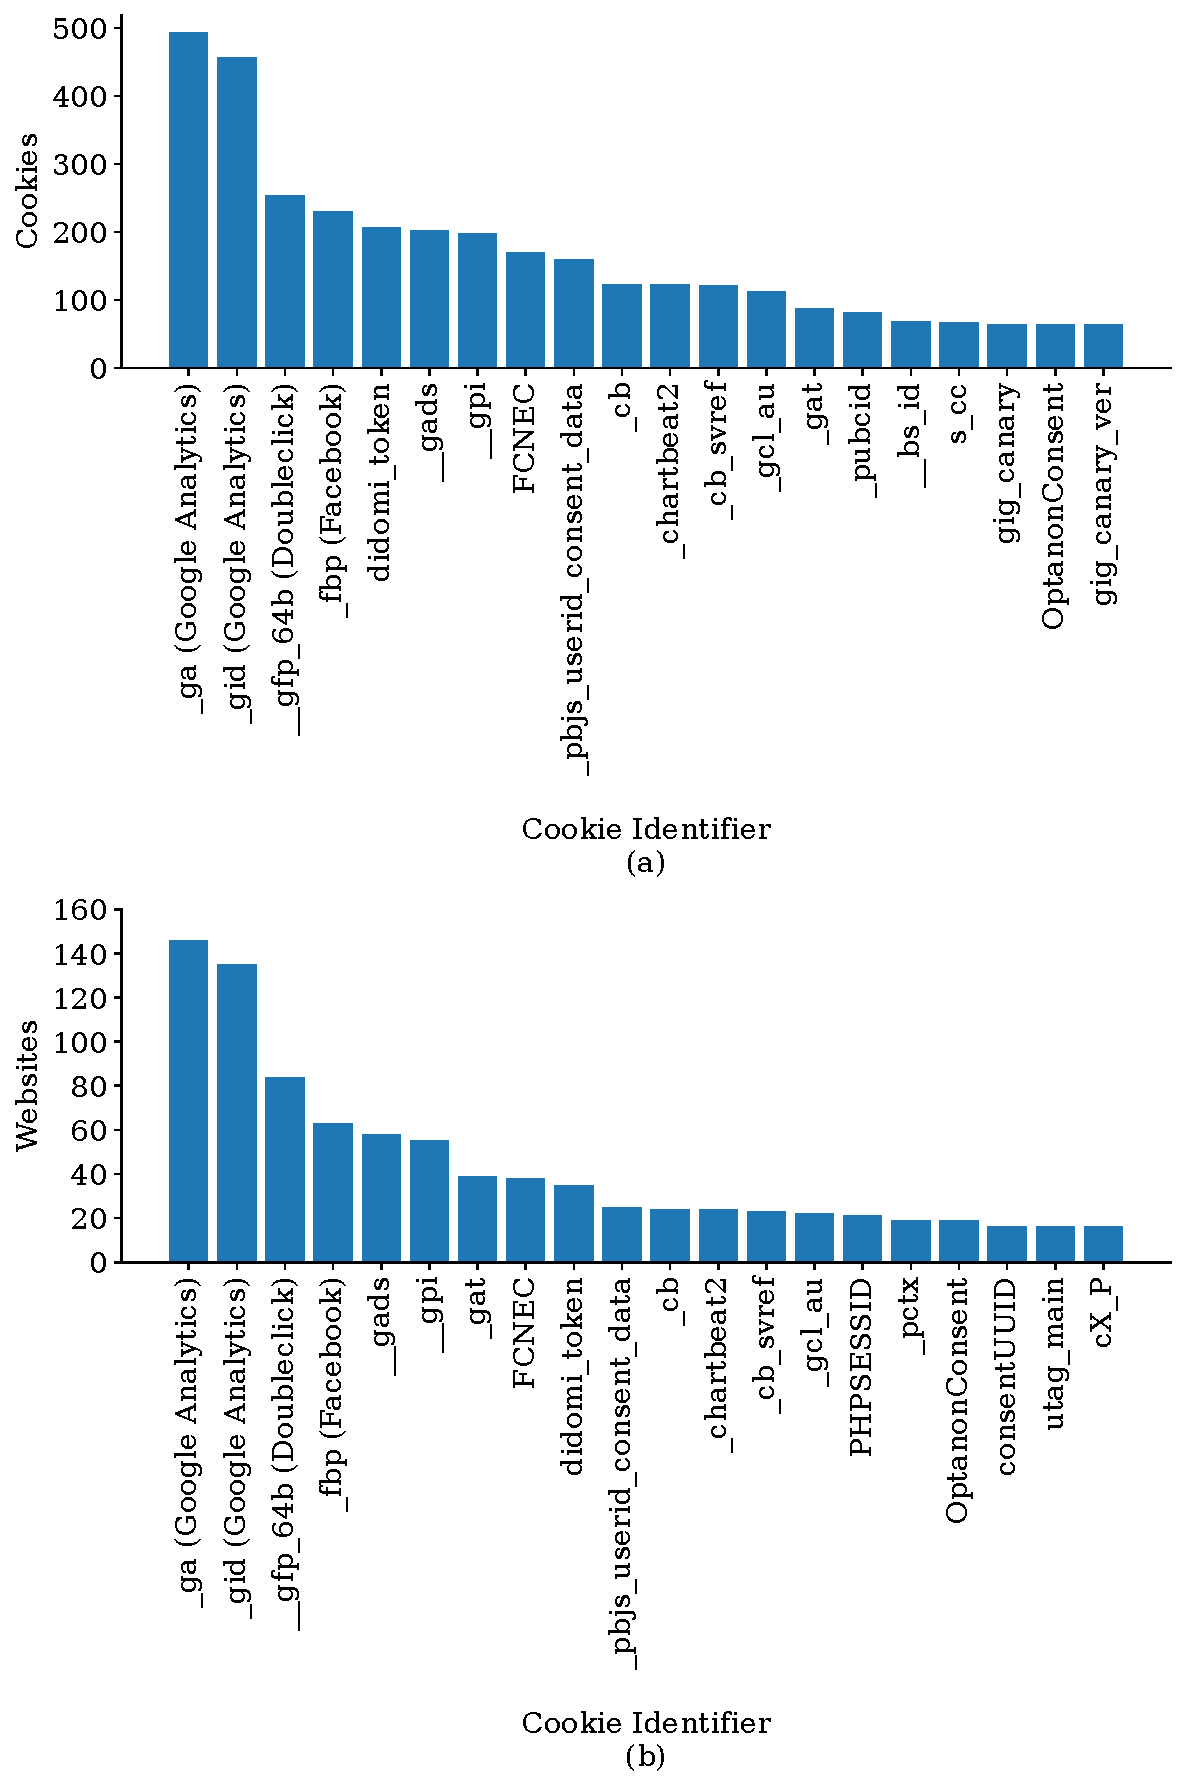
\includegraphics[width=\linewidth]{figures/cookie_analysis_combined.pdf}
    \caption{(a) Cookie identifier associated with the number of cookies. (b) Cookie identifier and number of website they are embedded.}
\label{fig:cookie_website}
\end{figure}
\end{center}


